\documentclass[aspectratio=169]{beamer}
\usepackage[utf8]{inputenc}
\usepackage[T1]{fontenc}
\usepackage{polski}
\usepackage{lmodern}
\usepackage{listings}
\usepackage{xcolor}
\usepackage{tikz}
\usetikzlibrary{shapes,arrows,positioning,trees}

\usetheme{Madrid}
\usecolortheme{default}

\lstset{
    language=Python,
    basicstyle=\ttfamily\footnotesize,
    keywordstyle=\color{blue},
    stringstyle=\color{red},
    commentstyle=\color{gray},
    showstringspaces=false,
    breaklines=true,
    frame=single,
    numbers=left,
    numberstyle=\tiny\color{gray},
    literate={@}{{@}}1 {\#}{{\#}}1
}

\setbeamertemplate{navigation symbols}{}
\setbeamertemplate{footline}{}

\title{Composite (Kompozyt)}
\subtitle{czyli jak policzyć orki Saurona bez zgłupienia}
\author{Wzorce projektowe -- laboratorium}
\date{5 grudnia 2025}

\begin{document}

\frame{\titlepage}

\begin{frame}{Wyobraź sobie...}
\begin{center}
\Large
Jesteś Sarumanem i musisz policzyć swoją armię przed atakiem na Helmowy Jar.
\end{center}

\pause

\vspace{0.5cm}

\begin{itemize}
    \item Masz \textbf{Armię Isengardu}...
    \pause
    \item ...która składa się z \textbf{Legionów}...
    \pause
    \item ...które składają się z \textbf{Oddziałów}...
    \pause
    \item ...które składają się z \textbf{Uruk-hai, Orków, Goblinów}...
\end{itemize}

\vspace{0.5cm}
\pause

\begin{center}
\textbf{Ile masz wojska?} \\
\vspace{0.3cm}
I jak to policzyć bez 47 zagnieżdżonych pętli?
\end{center}
\end{frame}

\begin{frame}[fragile]{Bez Composite -- pętle w pętlach w pętlach...}
\begin{lstlisting}[basicstyle=\ttfamily\tiny]
class Army:
    def __init__(self, name):
        self.name = name
        self.legions = []
    
    def total_strength(self):
        total = 0
        for legion in self.legions:
            for squad in legion.squads:
                for unit in squad.units:
                    total += unit.strength
        return total
    
    def count_units(self):
        count = 0
        for legion in self.legions:
            for squad in legion.squads:
                count += len(squad.units)
        return count
    
    def show_structure(self, indent=0):
        print("  " * indent + f"Armia: {self.name}")
        for legion in self.legions:
            print("  " * (indent+1) + f"Legion: {legion.name}")
            for squad in legion.squads:
                print("  " * (indent+2) + f"Oddzial: {squad.name}")
                for unit in squad.units:
                    print("  " * (indent+3) + f"- {unit.name}")
\end{lstlisting}

\textbf{Każda operacja = te same zagnieżdżenia!}
\end{frame}

\begin{frame}{Problem}
\begin{itemize}
    \item Masz \textbf{strukturę drzewiastą} (armia $\rightarrow$ legiony $\rightarrow$ oddziały $\rightarrow$ jednostki)
    \item \textbf{Każda operacja} wymaga tych samych zagnieżdżonych pętli
    \item Dodajesz nowy poziom (np. ,,Dywizja'')? \textbf{Zmieniasz WSZYSTKO}
    \item Chcesz policzyć siłę jednego oddziału? \textbf{Inny kod niż dla armii}
    \item Kod jest \textbf{kruchy} -- łatwo coś pominąć
\end{itemize}

\vspace{0.5cm}

\begin{center}
\Large
A gdyby \texttt{army.total\_strength()} \\
działało TAK SAMO jak \texttt{orc.total\_strength()}?
\end{center}

\vspace{0.5cm}

\begin{center}
\textbf{Rozwiązanie:} Composite Pattern
\end{center}
\end{frame}

\begin{frame}{Wzorzec Composite -- idea}
\begin{center}
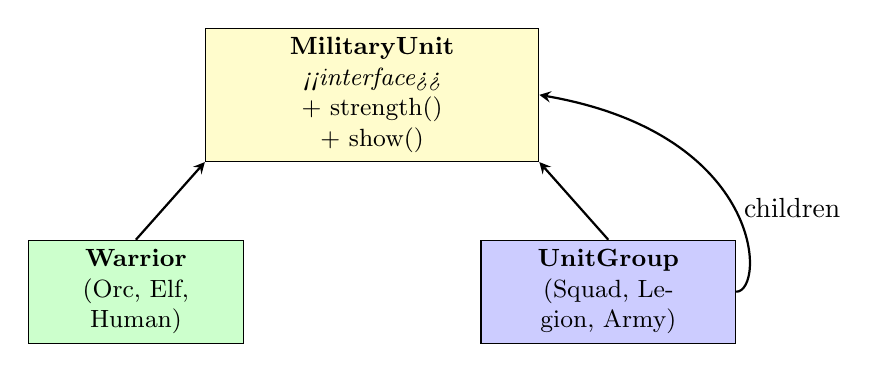
\begin{tikzpicture}[
    component/.style={rectangle, draw=black, fill=yellow!20, text width=4cm, text centered, minimum height=1.2cm, font=\small},
    leaf/.style={rectangle, draw=black, fill=green!20, text width=2.5cm, text centered, minimum height=1cm, font=\small},
    composite/.style={rectangle, draw=black, fill=blue!20, text width=3cm, text centered, minimum height=1cm, font=\small},
    arrow/.style={->, >=stealth, thick}
]
    % Component
    \node[component] (component) at (0, 2) {
        \textbf{MilitaryUnit}\\
        \textit{<<interface>>}\\
        + strength()\\
        + show()
    };
    
    % Leaf
    \node[leaf] (leaf) at (-3, -0.5) {
        \textbf{Warrior}\\
        (Orc, Elf, Human)
    };
    
    % Composite
    \node[composite] (composite) at (3, -0.5) {
        \textbf{UnitGroup}\\
        (Squad, Legion, Army)
    };
    
    % Arrows
    \draw[arrow] (leaf.north) -- (component.south west);
    \draw[arrow] (composite.north) -- (component.south east);
    
    % Self-reference for composite
    \draw[arrow] (composite.east) .. controls (5, -0.5) and (5, 1.5) .. node[right] {children} (component.east);
\end{tikzpicture}
\end{center}

\vspace{0.5cm}

\textbf{Idea:} Liść (pojedynczy wojownik) i Kompozyt (grupa) \textit{wyglądają tak samo} z zewnątrz!
\end{frame}

\begin{frame}[fragile]{Z Composite -- wspólny interfejs}
\begin{lstlisting}
from abc import ABC, abstractmethod

class MilitaryUnit(ABC):
    """Wspolny interfejs dla lisci i kompozytow"""
    
    @abstractmethod
    def strength(self) -> int:
        """Zwraca sile bojowa"""
        pass
    
    @abstractmethod
    def count(self) -> int:
        """Zwraca liczbe jednostek"""
        pass
    
    @abstractmethod
    def show(self, indent: int = 0) -> str:
        """Pokazuje strukture"""
        pass
\end{lstlisting}

\vspace{0.3cm}

\textbf{Kluczowe:} Ten sam interfejs dla orka i dla całej armii!
\end{frame}

\begin{frame}[fragile]{Z Composite -- Liść (pojedynczy wojownik)}
\begin{lstlisting}
class Warrior(MilitaryUnit):
    """Lisc -- pojedyncza jednostka bojowa"""
    
    def __init__(self, name: str, strength: int):
        self.name = name
        self._strength = strength
    
    def strength(self) -> int:
        return self._strength  # Po prostu zwraca swoja sile
    
    def count(self) -> int:
        return 1  # Jestem jeden!
    
    def show(self, indent: int = 0) -> str:
        return "  " * indent + f"- {self.name} (sila: {self._strength})"
\end{lstlisting}

\vspace{0.3cm}

\textbf{Liść} to koniec gałęzi -- nie ma dzieci.
\end{frame}

\begin{frame}[fragile]{Z Composite -- Kompozyt (grupa)}
\begin{lstlisting}[basicstyle=\ttfamily\tiny]
class UnitGroup(MilitaryUnit):
    """Kompozyt -- grupa jednostek (moze zawierac inne grupy!)"""
    
    def __init__(self, name: str):
        self.name = name
        self.children: List[MilitaryUnit] = []  # <-- MAGIA!
    
    def add(self, unit: MilitaryUnit):
        self.children.append(unit)
    
    def strength(self) -> int:
        # Sumuje sile WSZYSTKICH dzieci (rekurencyjnie!)
        return sum(child.strength() for child in self.children)
    
    def count(self) -> int:
        # Liczy WSZYSTKIE jednostki w poddrzewie
        return sum(child.count() for child in self.children)
    
    def show(self, indent: int = 0) -> str:
        lines = ["  " * indent + f"[{self.name}] (sila: {self.strength()}, jednostek: {self.count()})"]
        for child in self.children:
            lines.append(child.show(indent + 1))
        return "\n".join(lines)
\end{lstlisting}
\end{frame}

\begin{frame}[fragile]{Użycie -- budujemy Armię Mordoru!}
\begin{lstlisting}[basicstyle=\ttfamily\tiny]
# Pojedyncze jednostki (Liscie)
orc1 = Warrior("Grishnakh", 5)
orc2 = Warrior("Ugluk", 7)
uruk = Warrior("Lurtz", 15)
troll = Warrior("Jaskiniowy Troll", 50)

# Oddzialy (Kompozyty zawierajace Liscie)
scout_squad = UnitGroup("Zwiadowcy")
scout_squad.add(orc1)
scout_squad.add(orc2)

elite_squad = UnitGroup("Elita Uruk-hai")
elite_squad.add(uruk)
elite_squad.add(troll)

# Legion (Kompozyt zawierajacy Kompozyty!)
mordor_legion = UnitGroup("Legion Mordoru")
mordor_legion.add(scout_squad)
mordor_legion.add(elite_squad)

# Teraz MAGIA:
print(mordor_legion.strength())  # 77 (5+7+15+50) -- AUTOMATYCZNIE!
print(mordor_legion.count())     # 4 jednostki -- BEZ PETLI!
\end{lstlisting}
\end{frame}

\begin{frame}[fragile]{Magia Composite -- jednolite traktowanie}
\begin{lstlisting}
# Wszystko jest MilitaryUnit!
units = [orc1, scout_squad, mordor_legion]

for unit in units:
    # TEN SAM KOD dla orka, oddzialu i calego legionu!
    print(f"{unit.name}: sila={unit.strength()}, liczba={unit.count()}")
\end{lstlisting}

\vspace{0.5cm}

\textbf{Wynik:}
\begin{verbatim}
Grishnakh: sila=5, liczba=1
Zwiadowcy: sila=12, liczba=2
Legion Mordoru: sila=77, liczba=4
\end{verbatim}

\vspace{0.5cm}

\textbf{Klient nie musi wiedzieć} czy ma do czynienia z pojedynczą jednostką czy z całą armią!
\end{frame}

\begin{frame}[fragile]{Porównanie: Przed i Po}
\begin{columns}
\begin{column}{0.48\textwidth}
\textbf{Przed (pętle w pętlach):}
\begin{lstlisting}[basicstyle=\ttfamily\tiny]
def total_strength(army):
    total = 0
    for legion in army.legions:
        for squad in legion.squads:
            for unit in squad.units:
                total += unit.strength
    return total

def count_units(army):
    count = 0
    for legion in army.legions:
        for squad in legion.squads:
            count += len(squad.units)
    return count

# Dla pojedynczego orka? INNY KOD!
\end{lstlisting}

\textcolor{red}{[X]} Zagnieżdżenia\\
\textcolor{red}{[X]} Różny kod dla liścia/grupy\\
\textcolor{red}{[X]} Trudno dodać poziom
\end{column}
\begin{column}{0.48\textwidth}
\textbf{Po (Composite):}
\begin{lstlisting}[basicstyle=\ttfamily\tiny]
# Dla WSZYSTKIEGO ten sam interfejs!

army.strength()    # Cala armia
legion.strength()  # Legion
squad.strength()   # Oddzial
orc.strength()     # Jeden ork

# IDENTYCZNY KOD!
# Rekurencja zalatwia sprawe
\end{lstlisting}

\vspace{0.5cm}

\textcolor{green}{[OK]} Brak zagnieżdżonych pętli\\
\textcolor{green}{[OK]} Jednolity interfejs\\
\textcolor{green}{[OK]} Łatwo dodać poziom\\
\textcolor{green}{[OK]} Rekurencja robi robotę
\end{column}
\end{columns}
\end{frame}

\begin{frame}{Kiedy używać Composite?}
\begin{itemize}
    \item Masz \textbf{strukturę drzewiastą} (hierarchia część-całość)
    \item Chcesz traktować \textbf{pojedyncze elementy i grupy jednakowo}
    \item Operacje na grupie to \textbf{agregacja operacji na dzieciach}
    \item Chcesz \textbf{łatwo dodawać nowe poziomy} hierarchii
\end{itemize}

\vspace{0.5cm}

\textbf{Przykłady z życia:}
\begin{itemize}
    \item System plików (pliki i foldery)
    \item Menu w aplikacji (pozycje i podmenu)
    \item Organizacja firmy (pracownicy i działy)
    \item GUI (komponenty i kontenery)
    \item Drzewo DOM w HTML
\end{itemize}

\vspace{0.5cm}

\textbf{Trade-off:} Trudniej ograniczyć typy dzieci (np. ,,Legion nie może zawierać innego Legionu'')
\end{frame}

\begin{frame}{Dzisiaj na zajęciach}
\begin{enumerate}
    \item Dostaniecie kod symulatora armii Śródziemia (z pętlami): \\
    \texttt{https://github.com/refactor-or-die/lab06-war-of-the-ring}
    \item W parach zrefaktoryzujecie go używając wzorca Composite
    \item Stworzycie wspólny interfejs dla jednostek i grup
    \item Testy muszą przejść!
\end{enumerate}

\vspace{1cm}

\begin{center}
\Large
\textbf{Pytania?} \\
\vspace{0.5cm}
\normalsize
Jeśli nie -- to \texttt{git clone} i budujemy armie! \\
\vspace{0.3cm}
\small
\textit{,,Jedna armia, żeby wszystkimi rządzić...''}
\end{center}
\end{frame}

\end{document}